\subsubsection{Documentação Typedoc}
Durante a implementação desta ferramenta foi detetado que a categorização de documentação não se encontrava funcional devido a um problema encontrado pelos desenvolvedores da ferramenta, foi decidido então reduzir a versão da mesma para uma com a funcionalidade ativada, mas esta não se encontrava compatível com a versão mais atualizada de typescript, pelo que não foi possível explorar esta funcionalidade. Para contornar o problema foi então decidido explorar outra funcionalidade menos utilizada da ferramenta, esta funcionalidade permite converter qualquer documentação em módulos, estes módulos podem então ser categorizados, o problema destes módulos é que cria um modelo genérico do código não sendo fácilmente identificado as tipagens de scripts. Estes módulos permitem também a categorização dos mesmos permitindo assim um nível de organização da documentação gerada.

\newpage

\subsubsection{Documentação Swagger}
Apesar da ferramenta disponibilizar a geração automática de documentação a partir de comentários de código, foram encontrados alguns problemas com esta funcionalidade, acabando por não gerar a documentação, pelo que foi optado por manter a documentação manualmente com o ficheiro json. Esta ferramenta oferece diversas funcionalidades como autenticação, definição de estruturas de dados para os serviços e exemplos de respostas para os mesmos, ambas estas funcionalidades foram exploradas conseguindo assim um bom suporte de documentação para qualquer utilizador.

\begin{figure}[htb]
  \centering
  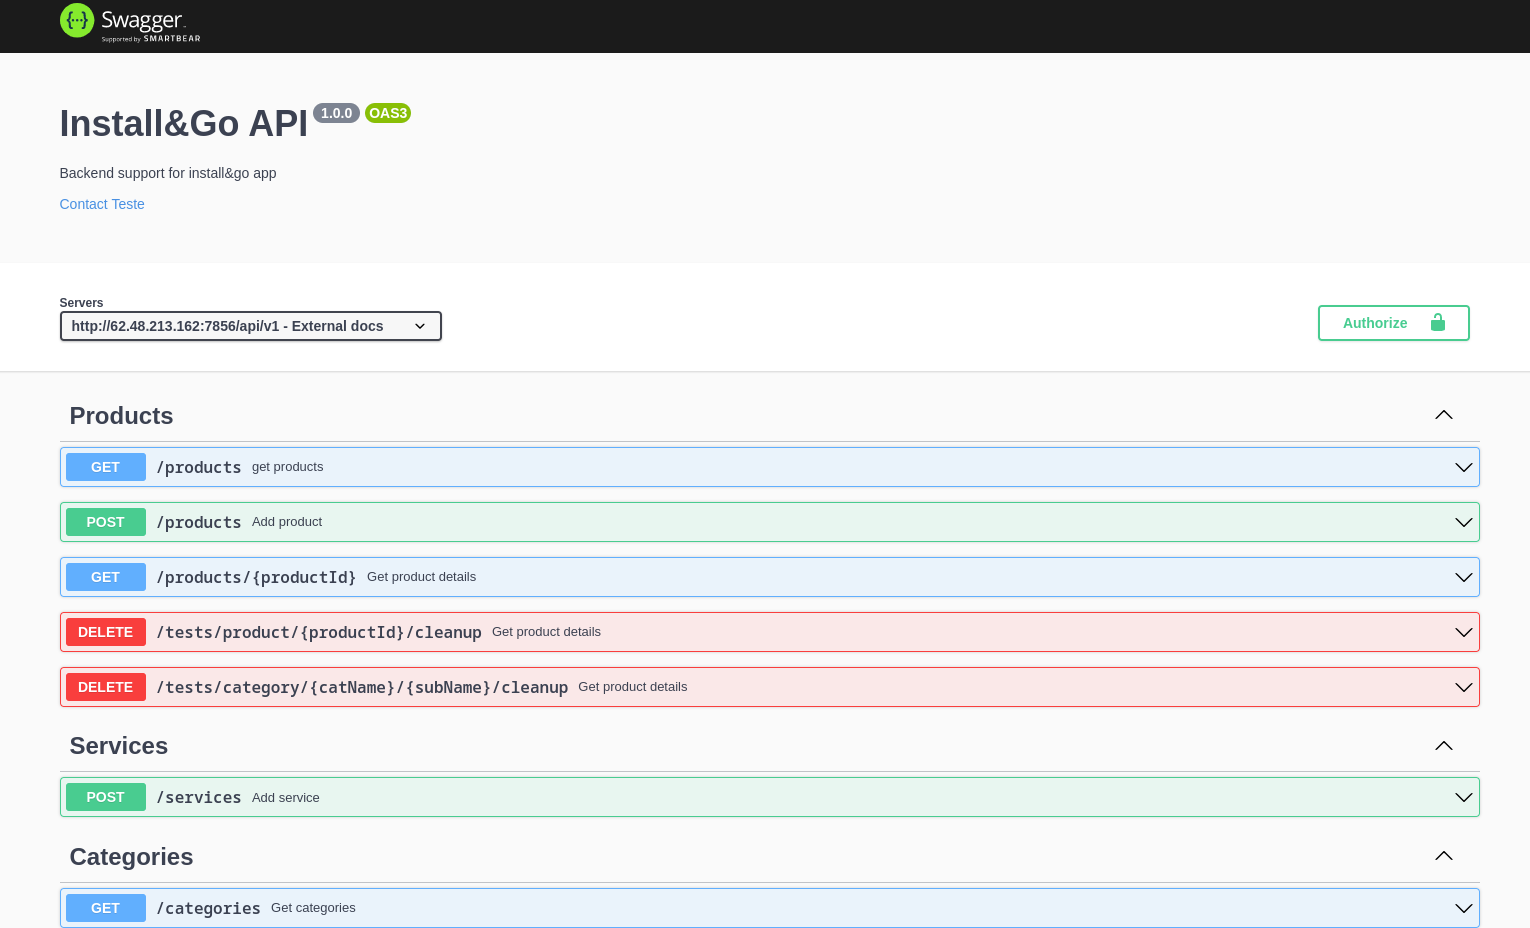
\includegraphics[width=0.6\textwidth]{images/implementacao/api/swagger_intro.png}
  \caption{Documentação swagger}
  \label{fig:66}
\end{figure}

\begin{figure}[htb]
  \centering
  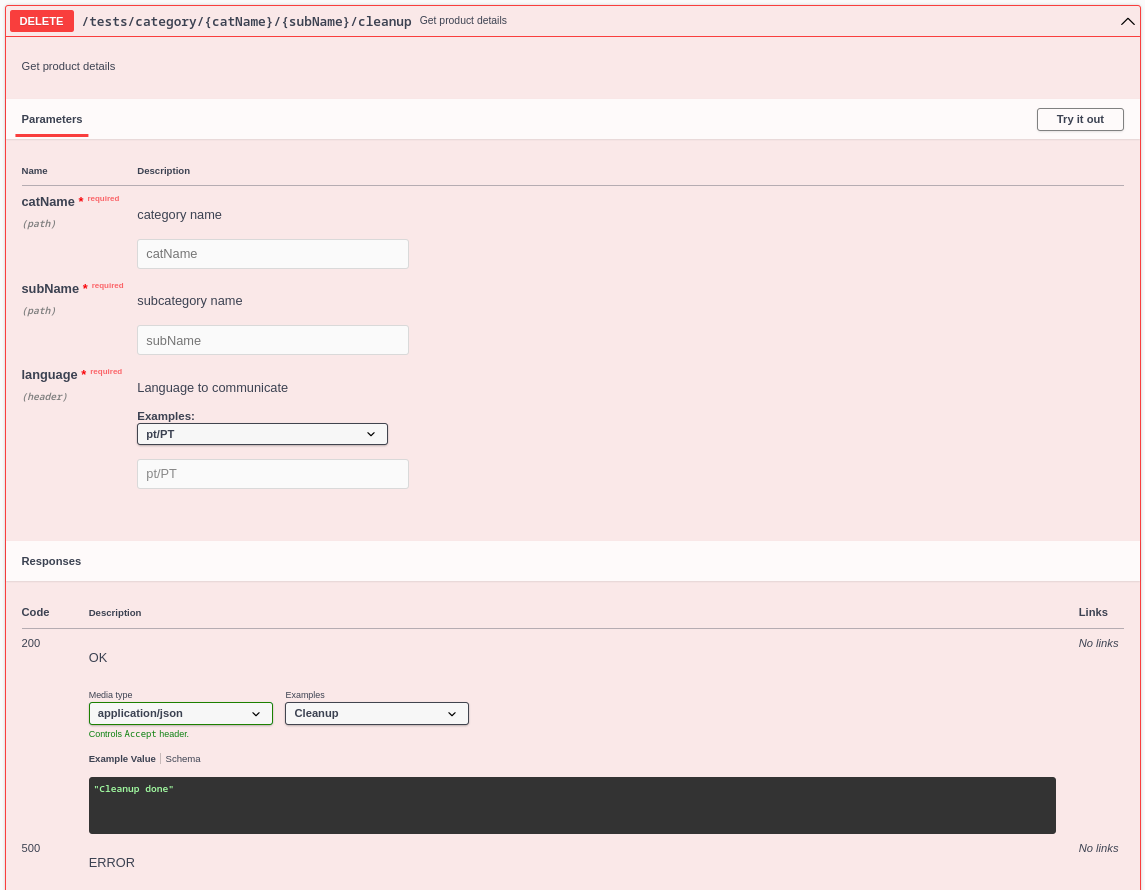
\includegraphics[width=0.6\textwidth]{images/implementacao/api/swagger_pedido.png}
  \caption{Exemplo de documentação de serviço}
  \label{fig:67}
\end{figure}